\section{Implementación}

\subsection{Arquitectura del sistema}
La arquitectura implementada sigue las mejores prácticas de desarrollo web moderno, integrando API REST con Spring Boot en el backend y React en el frontend. La persistencia se realiza en MySQL con un diseño relacional normalizado. La \cref{fig:correlacion_devops} muestra las estadísticas de emisión de certificados por mes.

\begin{figure}[htbp]
    \centering
    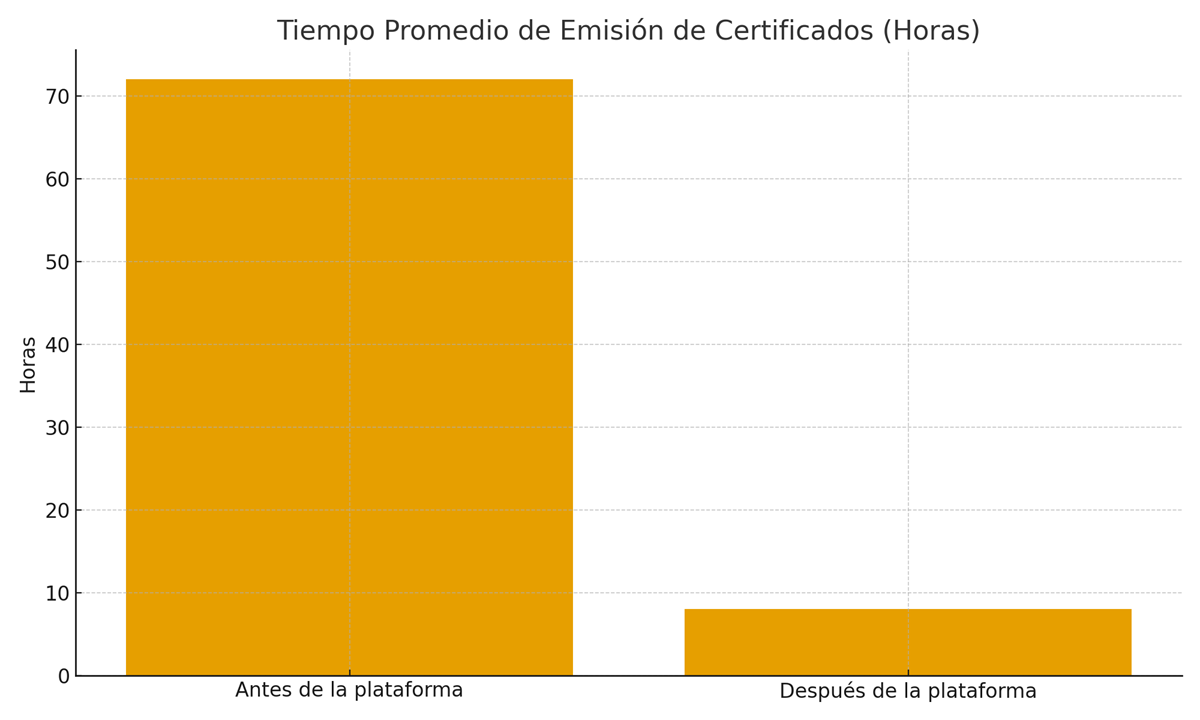
\includegraphics[width=0.46\textwidth]{graphics/emision_certificados.png}
    \caption{Emisión de certificados laborales por mes}
    \label{fig:correlacion_devops}
\end{figure}

\subsection{Módulos implementados}
La plataforma incluye los siguientes módulos principales:

\begin{itemize}
    \item \textbf{Autenticación y control de roles}: Sistema JWT para login, autorización por roles y renovación de tokens.
    \item \textbf{Gestión de empleados y contratos}: Fichas de empleados, contratos con fechas clave y renovaciones.
    \item \textbf{Registro de asistencia}: Entradas/salidas, cálculo de horas trabajadas y gestión de turnos.
    \item \textbf{Gestión de permisos e incapacidades}: Solicitudes con flujo de estados, adjuntos y bitácora.
    \item \textbf{Capacitaciones e inducción}: Asignación de contenidos, evaluaciones y seguimiento de avances.
    \item \textbf{Generación de certificados}: Certificados laborales con datos parametrizables.
    \item \textbf{Reportes y analítica}: Indicadores operativos y tendencias con visualizaciones.
    \item \textbf{Auditoría y seguridad}: Registro de acciones y control de integridad.
\end{itemize}

\subsection{Fragmento de código}
Ejemplo de implementación de un endpoint REST en Spring Boot:

\ifminted
\begin{minted}[linenos]{java}
@RestController
@RequestMapping("/api/empleados")
public class EmpleadoController {
    @Autowired
    private EmpleadoService empleadoService;

    @GetMapping("/{id}")
    public ResponseEntity<EmpleadoDTO> obtenerEmpleado(@PathVariable Long id) {
        EmpleadoDTO empleado = empleadoService.obtenerPorId(id);
        return ResponseEntity.ok(empleado);
    }
}
\end{minted}
\else
\begin{lstlisting}[language=Java]
@RestController
@RequestMapping("/api/empleados")
public class EmpleadoController {
    @Autowired
    private EmpleadoService empleadoService;

    @GetMapping("/{id}")
    public ResponseEntity<EmpleadoDTO> obtenerEmpleado(@PathVariable Long id) {
        EmpleadoDTO empleado = empleadoService.obtenerPorId(id);
        return ResponseEntity.ok(empleado);
    }
}
\end{lstlisting}
\fi

\subsection{Tecnologías utilizadas}
La selección de tecnologías se basó en madurez, comunidad y adecuación al dominio. La \cref{tab:frameworks} presenta una comparación detallada de los frameworks evaluados.

\input{tables/frameworks_comparison.tex}